\section*{Competencia}
\addcontentsline{toc}{section}{Competencia}

A continuación describiremos los competidores más directos de nuestro proyecto.

\subsection*{BBVA Bconomy}
\addcontentsline{toc}{subsection}{BBVA Bconomy}
BBVA Bconomy es una plataforma creada por el Banco Bilbao Vizcana Argentaria que busca facilitar la vida de los clientes poniendo a disposición la información posible para tomar sus propias decisiones financieras. Esta herramienta, hecha en el año 2017, tiene como objetivo permitir disponer un diagnóstico personalizado acerca del estado de su salud financiera. BBVA Bconomy ofrece medir la evolución de los ingresos y gastos de los clientes en 4 variables, ahorro mensual, libertad económica, el gasto destinado a vivienda y gastos por préstamos o pagos aplazados por tarjeta \parencite{BBVA03}.

\begin{figure}[H]
	\centering
	
\includegraphics[width=10cm]{Imagenes/LogoBConomy.png}
	\caption[{Logotipo de BBVA Bconomy.}]{\centering Logotipo de BBVA Bconomy. \textit{Fuente:} Entre nosotros, BBVA, 2024, Origen: https://view.ceros.com/avalon/bbva-entre-nosotros-13/p/4} 
	\label{fig:logobconomy}
\end{figure}

\subsection*{Fintonic}
\addcontentsline{toc}{subsection}{Fintonic}
Fintonic es una aplicación de origen español la cual permite al usuario llevar un control de su dinero de forma visual e intuitiva, permitiendo agrupar gastos, controlar el dinero a partir de diferentes bancos, recibir avisos, etc. Realizando un exhaustivo registro y control sobre los gastos de cada usuario \parencite{EIP01}.

\begin{figure}[H]
	\centering
	
\includegraphics[width=15cm]{Imagenes/LogoFintonic.png}
	\caption[{Logotipo de Fintonic.}]{\centering Logotipo de BBVA Bconomy. \textit{Fuente:} Qué es Fintonic y cómo nos puede ayudar en el control financiero, Ruiz R., 2019, Origen: https://eiposgrados.com/blog-direccion-financiera/que-es-fintonic-y-como-nos-puede-ayudar-en-el-control-financiero/} 
	\label{fig:fintonic}
\end{figure}

\subsection*{Nequi}
\addcontentsline{toc}{subsection}{Nequi}
Nequi es una plataforma de banco totalmente digital, creada en el año 2016 como un proyecto corporativo de Bancolombia. Funciona bajo un modelo de Fintech con una apuesta de ser 100\% digital, buscando facilitar la relación entre las personas con el dinero, la banca y reducir la brecha del acceso al sistema financiero, actualmente es el sistema bancario digital con mayor cantidad de usuarios en Colombia \parencite{Pragma01}.

\begin{figure}[H]
	\centering
	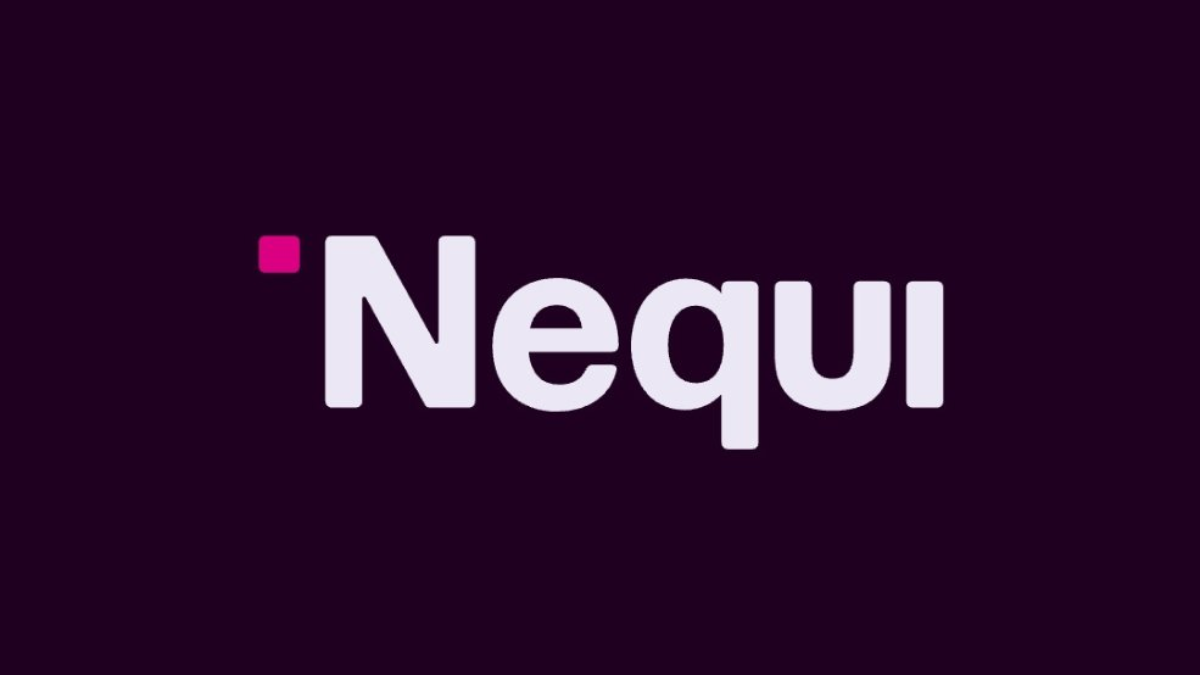
\includegraphics[width=10cm]{Imagenes/LogoNequi.png}
	\caption[{Logotipo de Nequi.}]{\centering Logotipo de Nequi. \textit{Fuente:} Nequi renueva su imagen: cuenta con más de 17,5 millones de clientes en Colombia, Neira J. G., Valora Analitik, 2023, Origen: https://www.valoraanalitik.com/nequi-renueva-su-imagen-cuenta-con-mas-de-17-5-millones-de-clientes-en-colombia/} 
	\label{fig:logonequi}
\end{figure} 